\chapter{Analysis}

\section{Photometry}
\label{analysis_phot}

\subsection{Rapid Oscillations in photometric lightcurves}
\label{ro_phot_lc}
Photometry lightcurves from all 4 nights were flattened using the method described in section \ref{flat_section}. Periodograms were then calculated for these in order to identify any DNOs, lpDNOs and QPOs. Periodograms were calculated using the algorithm in \cite{kurtz_ft}. See figures \ref{S7651}, \ref{S7655} and \ref{S7659}. The DNO ($\sim3600$ cycles/day) and lpDNO($\sim1000$ cycles/day) spikes in the periodogram can clearly be seen in run S7651 and S7655. On the third night (Run \#S7659) the DNOs and lpDNOs were not visible. Run \# S7661 were hampered by cloud and only a very short observing run was possible. The data from this run were not used in any further analyses. The DNOs, lpDNOs and QPOs identified in the photometric lightcurves are shown in table \ref{RO_table}.

\begin{table}
\begin{scriptsize}
 
\centering
% use packages: array,supertabular
\begin{tabular}{ccccccc}
\hline \hline\\
Run    & DNO period & DNO freq      & lpDNO period & lpDNO freq     & QPO (s)\\ 
       & (s)        &  (cycles/day) &  (s)         &  (cycles/day)  &        \\ 
\\\hline \\
S7651  & 24.27, 24.15 & 3559.19, 3576.91 &  89.97 &  960.31  &  \\ 
S7655  & 23.76 & 3636.95 & 104.19 & 829.22 & \\ 
S7659  & --& --& -- &&\\ 
S7661  & -- & -- & -- &&\\\\
\hline
\end{tabular}

\caption[Rapid Oscillations in photometry]{Rapid Oscillations in photometry.}
\label{RO_table}
\end{scriptsize}
\end{table}



\subsubsection{Run S7651}

The periodogram of the flattened lightcurve of run S7651 (figure \ref{S7651}) shows evidence for a double DNO with periods of 24.27s and 24.15s (table \ref{RO_table}). The $O-C$ diagrams (figures \ref{OC_S7651_1} and \ref{OC_S7651_2} ) show evidence of DNOs with changing phases. Examining the spectrogram (figure \ref{trailed_ft_S7651}) for this run, the DNO seems to show only a single frequency. The resolution of the spectrogram is not high enough to discern these different DNOs since their periods are very similar (table \ref{RO_table}). The spectrogram shows a changing frequency of the DNO during eclipse. This is most probably due to a phase shift instead of a change in frequency of the actual oscillation.

There is evidence for an increase in the DNO amplitude in the $O-C$ diagrams and the spectrogram for this run. The same phenomenon is observed in run S7655, discussed in the following section.

The spectrogram was calculated from the flattened lightcurve of this run.



\begin{figure}
 \centering
 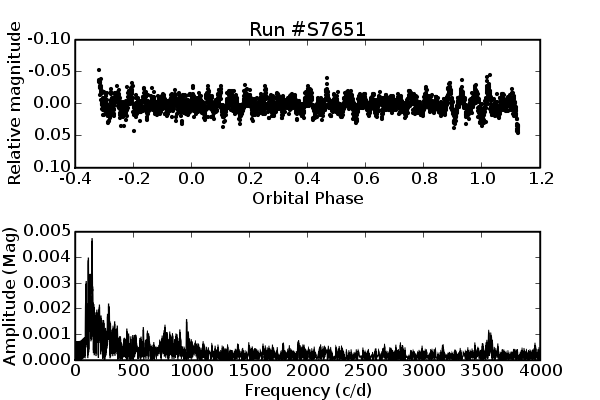
\includegraphics[width = 0.8\columnwidth, bb=0 0 600 400]{images/S7651.png}
 % vel_ew.png: 1179666x1179666 pixel, 0dpi, infxinf cm, bb=0 0 600 400
 \caption{Flattened lightcurve and periodogram for run S7651.}
 \label{S7651}
\end{figure}


\begin{figure}
 \centering
 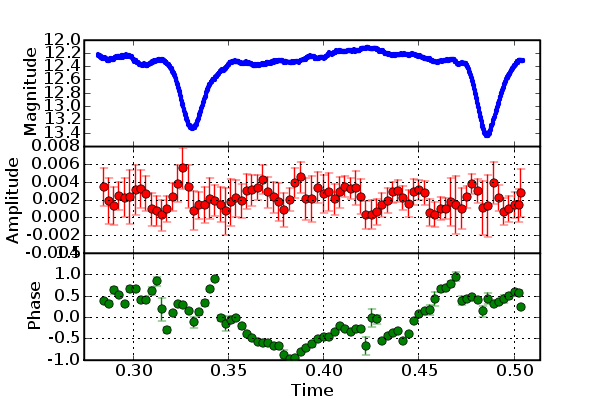
\includegraphics[width = 0.8\columnwidth, bb=0 0 600 400]{images/run1_flat.png}
 % vel_ew.png: 1179666x1179666 pixel, 0dpi, infxinf cm, bb=0 0 600 400
 \caption[$O-C$ diagram of the 3559.19 cycles/day DNO of run S7651.]{$O-C$ diagram of the 3559.19 cycles/day DNO of run S7651. Diagram was calculated using 20 cycles with 50 \% overlap.}
 \label{OC_S7651_1}
\end{figure}


\begin{figure}
 \centering
 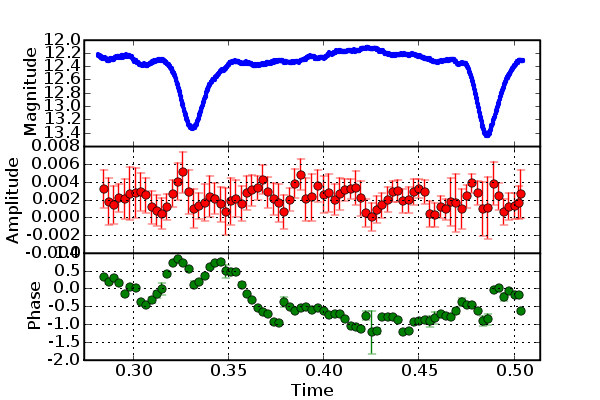
\includegraphics[width = 0.8\columnwidth, bb=0 0 600 400]{images/run1_flat_2.png}
 % vel_ew.png: 1179666x1179666 pixel, 0dpi, infxinf cm, bb=0 0 600 400
 \caption[$O-C$ diagram of the 3576.91 cycles/day DNO of run S7651.]{$O-C$ diagram of the 3576.91 cycles/day DNO of run S7651. Diagram was calculated using 20 cycles with 50 \% overlap.}
 \label{OC_S7651_2}
\end{figure}


\begin{figure}
 \centering
 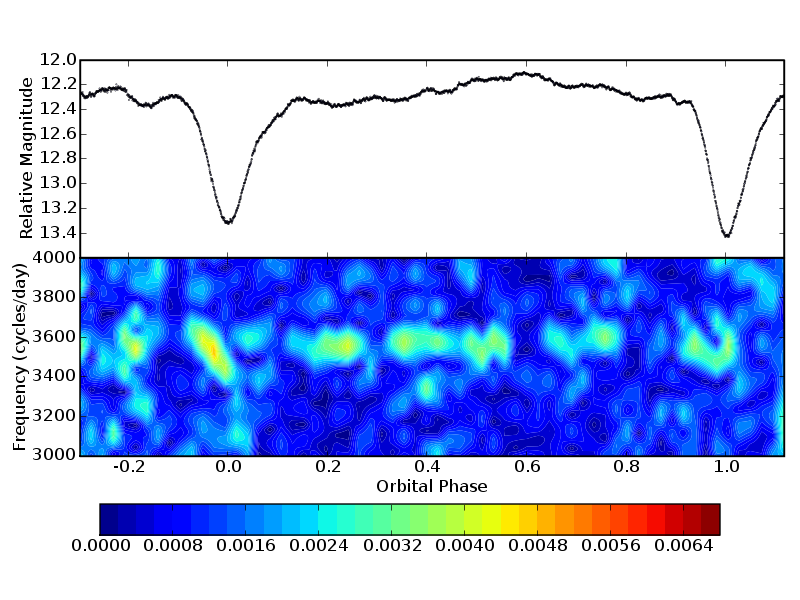
\includegraphics[width = 0.8\columnwidth, bb=0 0 800 600]{images/trailed_FT_S7651_colour.png}
 % vel_ew.png: 1179666x1179666 pixel, 0dpi, infxinf cm, bb=0 0 600 400
 \caption[Raw lightcurve and spectrogram for run S7651.]{Raw lightcurve and spectrogram for run S7651. The spectrogam was calculated from the flattened lightcurve of this run using 600s segments with 50\% overlap.}
 \label{trailed_ft_S7651}
\end{figure}

\subsubsection{Run S7655}

The periodogram (figure \ref{S7655}) of the flattened lightcurve of this run shows a very strong peak at 3636.9 cycles/day (period of 23.8s). The $O-C$ diagram (figure \ref{OC_S7655}) supports a stable oscillation at this period. There is also a marked increase in the DNO amplitude near HJD $\sim0.41$ and $\sim0.57$ which is approximately the times of mid-eclipse. This notion is also supported by the spectrogram of this run (figure \ref{trailed_ft_S7655}). This amplitude increase is probably due to the decrease in non-oscillating light from the accretion disk during eclipse, which enables us to see the DNO source more clearly. The spectrogram shows the same ``frequency'' change seen in run S7651. This phase change can be seen in the $O-C$ diagrams that is concentrated on the times of eclipse (figures \ref{OC_S7655_eclipse1} and \ref{OC_S7655_eclipse2}).



The spectrogram was calculated from the flattened lightcurve of this run.



% $O-C$ diagrams (section \ref{ominc_section}) were calculated to track the changes in the DNOs, lpDNOs and QPOs. These are shown for run S7651 in figures \ref{OC_S7651_1} and \ref{OC_S7651_2} and for run S7655 in figure \ref{OC_S7655}.


\begin{figure}
 \centering
 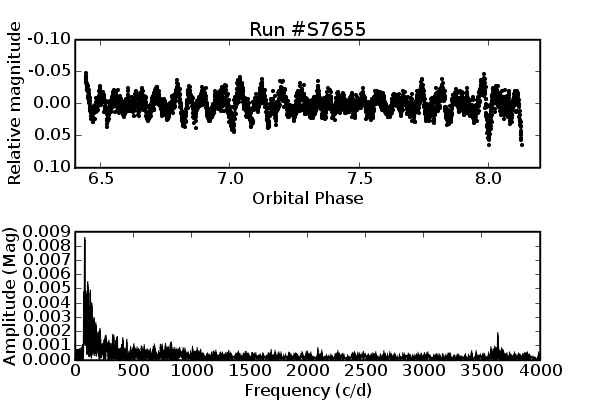
\includegraphics[width = 0.8\columnwidth, bb=0 0 600 400]{images/S7655.png}
 % vel_ew.png: 1179666x1179666 pixel, 0dpi, infxinf cm, bb=0 0 600 400
 \caption{Flattened lightcurve and periodogram for run S7655.}
 \label{S7655}
\end{figure}

\begin{figure}
 \centering
 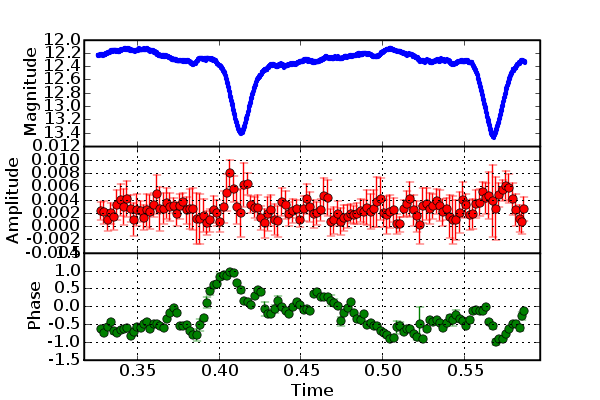
\includegraphics[width = 0.8\columnwidth, bb=0 0 600 400]{images/run2_flat.png}
 % vel_ew.png: 1179666x1179666 pixel, 0dpi, infxinf cm, bb=0 0 600 400
 \caption[$O-C$ diagram of the 3636.95 cycles/day DNO of run S7655.]{$O-C$ diagram of the 3636.95 cycles/day DNO of run S7655. Diagram was calculated using 20 cycles with 50 \% overlap.}
 \label{OC_S7655}
\end{figure}

\begin{figure}
 \centering
 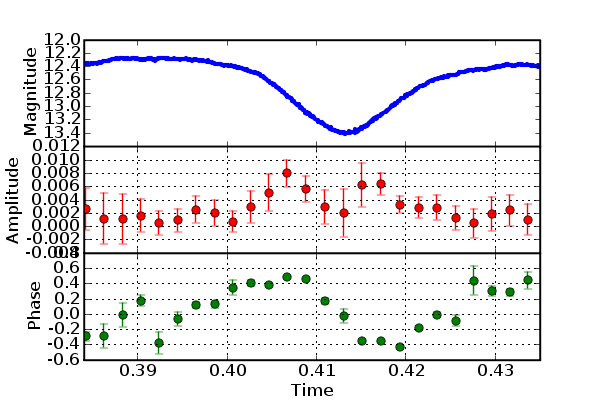
\includegraphics[width = 0.8\columnwidth, bb=0 0 600 400]{images/run2_eclipse1_oc.png}
 % vel_ew.png: 1179666x1179666 pixel, 0dpi, infxinf cm, bb=0 0 600 400
 \caption[$O-C$ diagram first eclipse of the 3636.95 cycles/day DNO of run S7655.]{$O-C$ diagram first eclipse of the 3636.95 cycles/day DNO of run S7655. Diagram was calculated using 15 cycles with 50 \% overlap.}
 \label{OC_S7655_eclipse1}
\end{figure}

\begin{figure}
 \centering
 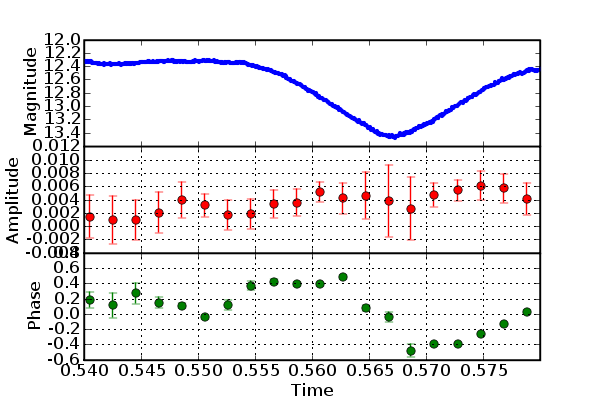
\includegraphics[width = 0.8\columnwidth, bb=0 0 600 400]{images/run2_eclipse2_oc.png}
 % vel_ew.png: 1179666x1179666 pixel, 0dpi, infxinf cm, bb=0 0 600 400
 \caption[$O-C$ diagram of the second eclipse of the 3636.95 cycles/day DNO of run S7655.]{$O-C$ diagram of the second eclipse of the 3636.95 cycles/day DNO of run S7655. Diagram was calculated using 15 cycles with 50 \% overlap.}
 \label{OC_S7655_eclipse2}
\end{figure}

\begin{figure}
 \centering
 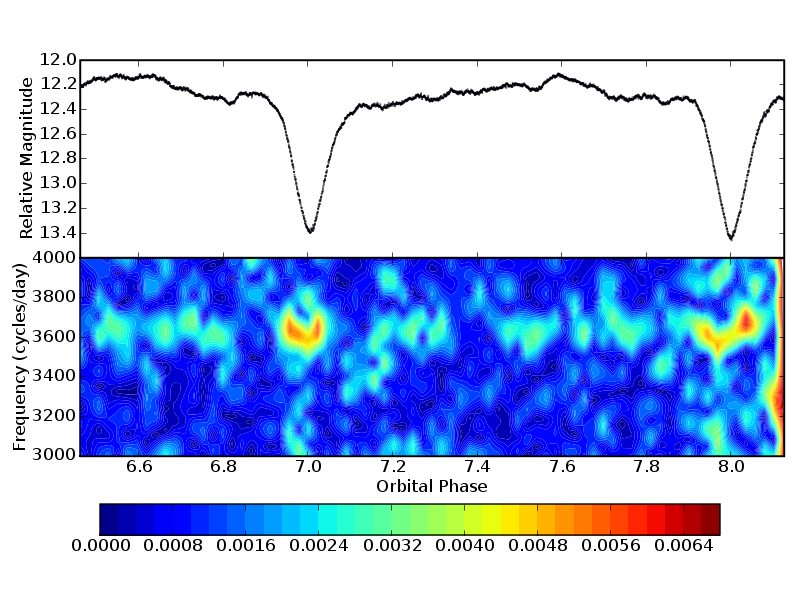
\includegraphics[width = 0.8\columnwidth, bb=0 0 800 600]{images/trailed_FT_S7655_colour.png}
 % vel_ew.png: 1179666x1179666 pixel, 0dpi, infxinf cm, bb=0 0 600 400
 \caption[Raw lightcurve and spectrogram for run S7655.]{Raw lightcurve and spectrogram for run S7655. The spectrogam was calculated from the flattened lightcurve of this run using 600s segments with 50\% overlap.}
 \label{trailed_ft_S7655}
\end{figure}






\begin{figure}
 \centering
 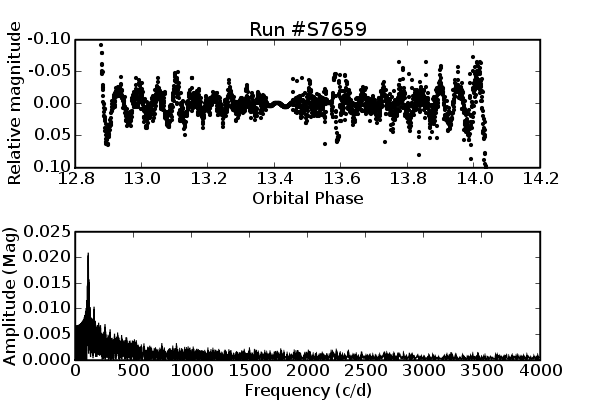
\includegraphics[width = 0.8\columnwidth, bb=0 0 600 400]{images/S7659.png}
 % vel_ew.png: 1179666x1179666 pixel, 0dpi, infxinf cm, bb=0 0 600 400
 \caption{Flattened lightcurve and periodogram for run S7659.}
 \label{S7659}
\end{figure}




\section{Spectroscopy}

\begin{figure}
 \centering
 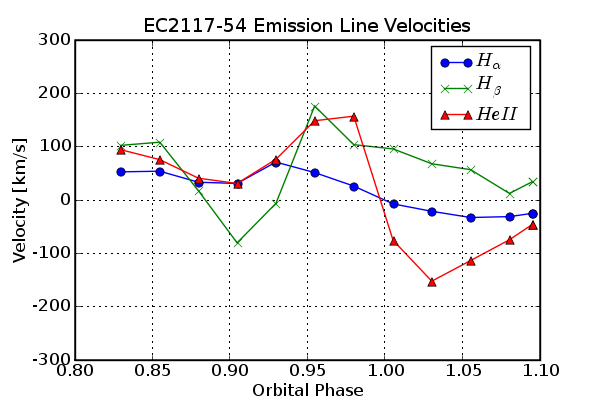
\includegraphics[width = 0.8\columnwidth, bb=0 0 600 400]{images/vel_gauss.png}
 % vel_ew.png: 1179666x1179666 pixel, 0dpi, infxinf cm, bb=0 0 600 400
 \caption{Line Velocities obtained by fitting gaussians.}
 \label{vel_gauss}
\end{figure}


\begin{figure}
 \centering
 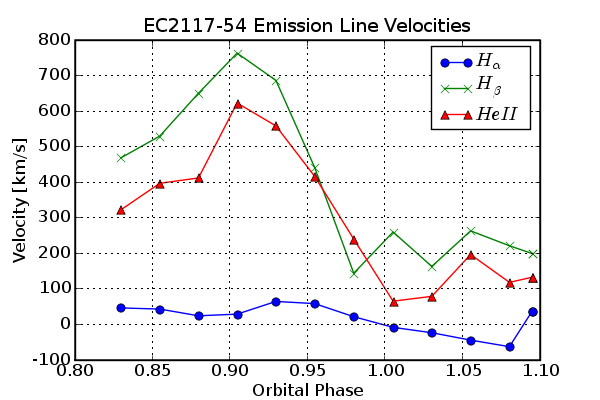
\includegraphics[width = 0.8\columnwidth, bb=0 0 600 400]{images/vel_ew.png}
 % vel_ew.png: 1179666x1179666 pixel, 0dpi, infxinf cm, bb=0 0 600 400
 \caption{Line Velocities obtained using equivalent width measurements.}
 \label{vel_ew}
\end{figure}


\begin{figure}
 \centering
 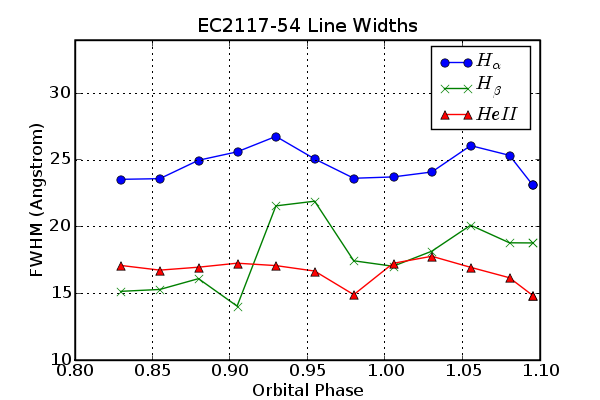
\includegraphics[width = 0.8\columnwidth, bb=0 0 600 400]{images/lw_gauss.png}
 % vel_ew.png: 1179666x1179666 pixel, 0dpi, infxinf cm, bb=0 0 600 400
 \caption{Line widths obtained using fitted gaussians.}
 \label{lw_gauss}
\end{figure}


\begin{figure}
 \centering
 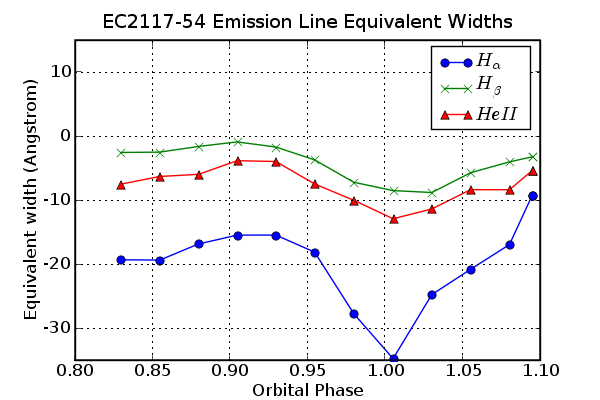
\includegraphics[width = 0.8\columnwidth, bb=0 0 600 400]{images/lw_ew.png}
 % vel_ew.png: 1179666x1179666 pixel, 0dpi, infxinf cm, bb=0 0 600 400
 \caption{Line widths obtained using equivalent width measurements.}
 \label{lw_ew}
\end{figure}



\begin{figure}
 \centering
 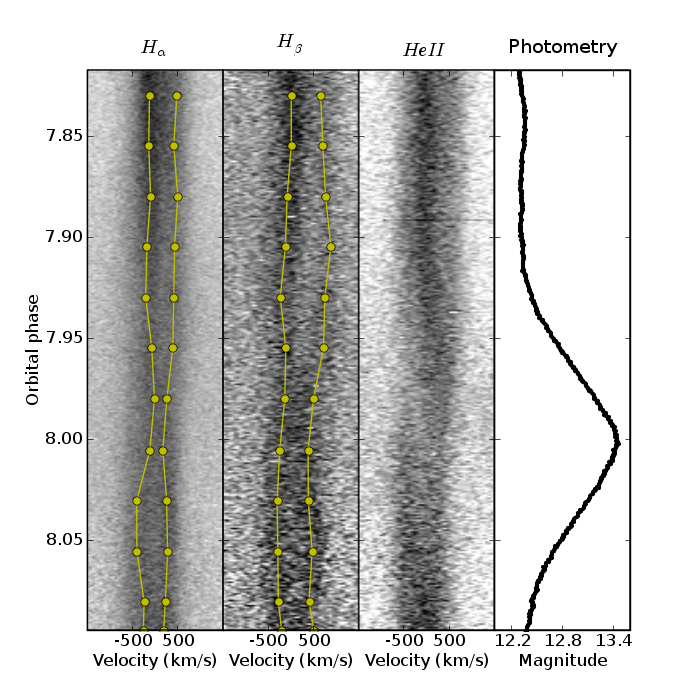
\includegraphics[width = \columnwidth, bb=0 0 800 800]{images/specgram.png}
 % specgramHa.png: 1179666x1179666 pixel, 0dpi, infxinf cm, bb=
 \caption{Trailed spectrogram around the $H_{\alpha}$,$H_{\beta}$ and \textit{HeII} lines.}
 \label{specgram}
\end{figure}





